\documentclass[fullscreen=true, bookmarks=true, hyperref={pdfencoding=unicode}]{beamer}
\usepackage[utf8]{inputenc}                                % Кодировка
\usepackage[english,russian]{babel}                        % Переносы
\usepackage{xcolor}                                        % Работа с цветом
\usepackage{amsmath,amssymb,amsfonts}                      % Символы АМО
\usepackage{graphicx}                                      % Графика
\usepackage[labelsep=period]{caption}                      % Разделитель в подписях к рисункам и таблицам
\usepackage{hhline}                                        % Для верстки линий в таблицах
\usepackage{tikz}                                          % Для простых рисунков в документе
\usepackage{fancybox}                                      % Пакет для отрисовки рамок
\usepackage{verbatim}                                      % Для вставки кода в презентацию
\usepackage{animate}                                       % Для вставки видео в презентацию
\usepackage{xmpmulti}                                      % Для вставки gif в презентацию
\usepackage{multirow}
\usepackage{mathrsfs}
\usepackage[normalem]{ulem}

\usetikzlibrary{arrows, snakes, backgrounds}                 % Для отрисовки стрелок
\usetikzlibrary{positioning, fit, arrows.meta, shapes, calc}
% used to avoid putting the same thing several times...
% Command \empt{var1}{var2}
\newcommand{\empt}[2]{$#1^{\langle #2 \rangle}$}

\graphicspath{{images/}}                                   % Путь до рисунков
\setbeamertemplate{caption}[numbered]                      % Включение нумерации рисунков

\definecolor{links}{HTML}{2A1B81}                          % blue for url links
\hypersetup{colorlinks,linkcolor=,urlcolor=links}          % nothing for others

\usetheme{Boadilla}
\usecolortheme{whale}

\usepackage{minted}

% \setbeameroption{show notes}
\setbeameroption{hide notes}
% \setbeameroption{show only notes}

\title{Lecture 12. Intro to Reinforcement Learning}
\author{Alex Avdyushenko}
\institute{Kazakh-British Technical University}
\date{November 26, 2022}
\titlegraphic{
\includegraphics[keepaspectratio,width=0.4\textwidth]{logo_kbtu.png}}

\begin{document}
%\unitlength=2mm

% выводим заглавие
\begin{frame}
\transdissolve[duration=0.2]
\titlepage
\end{frame}

\note{Good afternoon, dear students. Today we are going to talk about reinforcement learning, it is a slightly separate topic that is not directly related to deep learning, but is included in machine learning of course. It is quite possible to read a semester course on it, but we will limit ourselves to today's one lecture.}

\begin{frame}
  \frametitle{Five-minutes block}
  \pause
  \begin{itemize}
    \item Describe (or draw) the general architecture of the autoencoder
    \item What is the main advantage of the self-supervised learning method?
    \item Please, write down GAN loss functions
  \end{itemize}
\end{frame}

\note{Ok, and as usual now we have five-minutes block. The last one in our course. So prepare yourself and send right answers to me in five minutes.}

\begin{frame}
  \frametitle{Problem Statement}

  \begin{itemize}
    \item Up to this point, we either restored the function from the training set $(X, Y)$ (supervised learning) or searched for the structure in the set of objects $X$ (unsupervised learning)
    \pause
    \item But how does learning work in real world? Usually we do some action and get the result, gradually learning
  \end{itemize}
\end{frame}

\note{Great, let's go on and let me remind you, that up to this point, we found the appropriate function f, based on the training set. And it is called supervised learning. Or also we found the inner structure in the set of objects, you know, texts or images, and it is called unsupervised learning, when we haven't answers y.}

\begin{frame}
  \frametitle{Real world}

  \begin{center}
    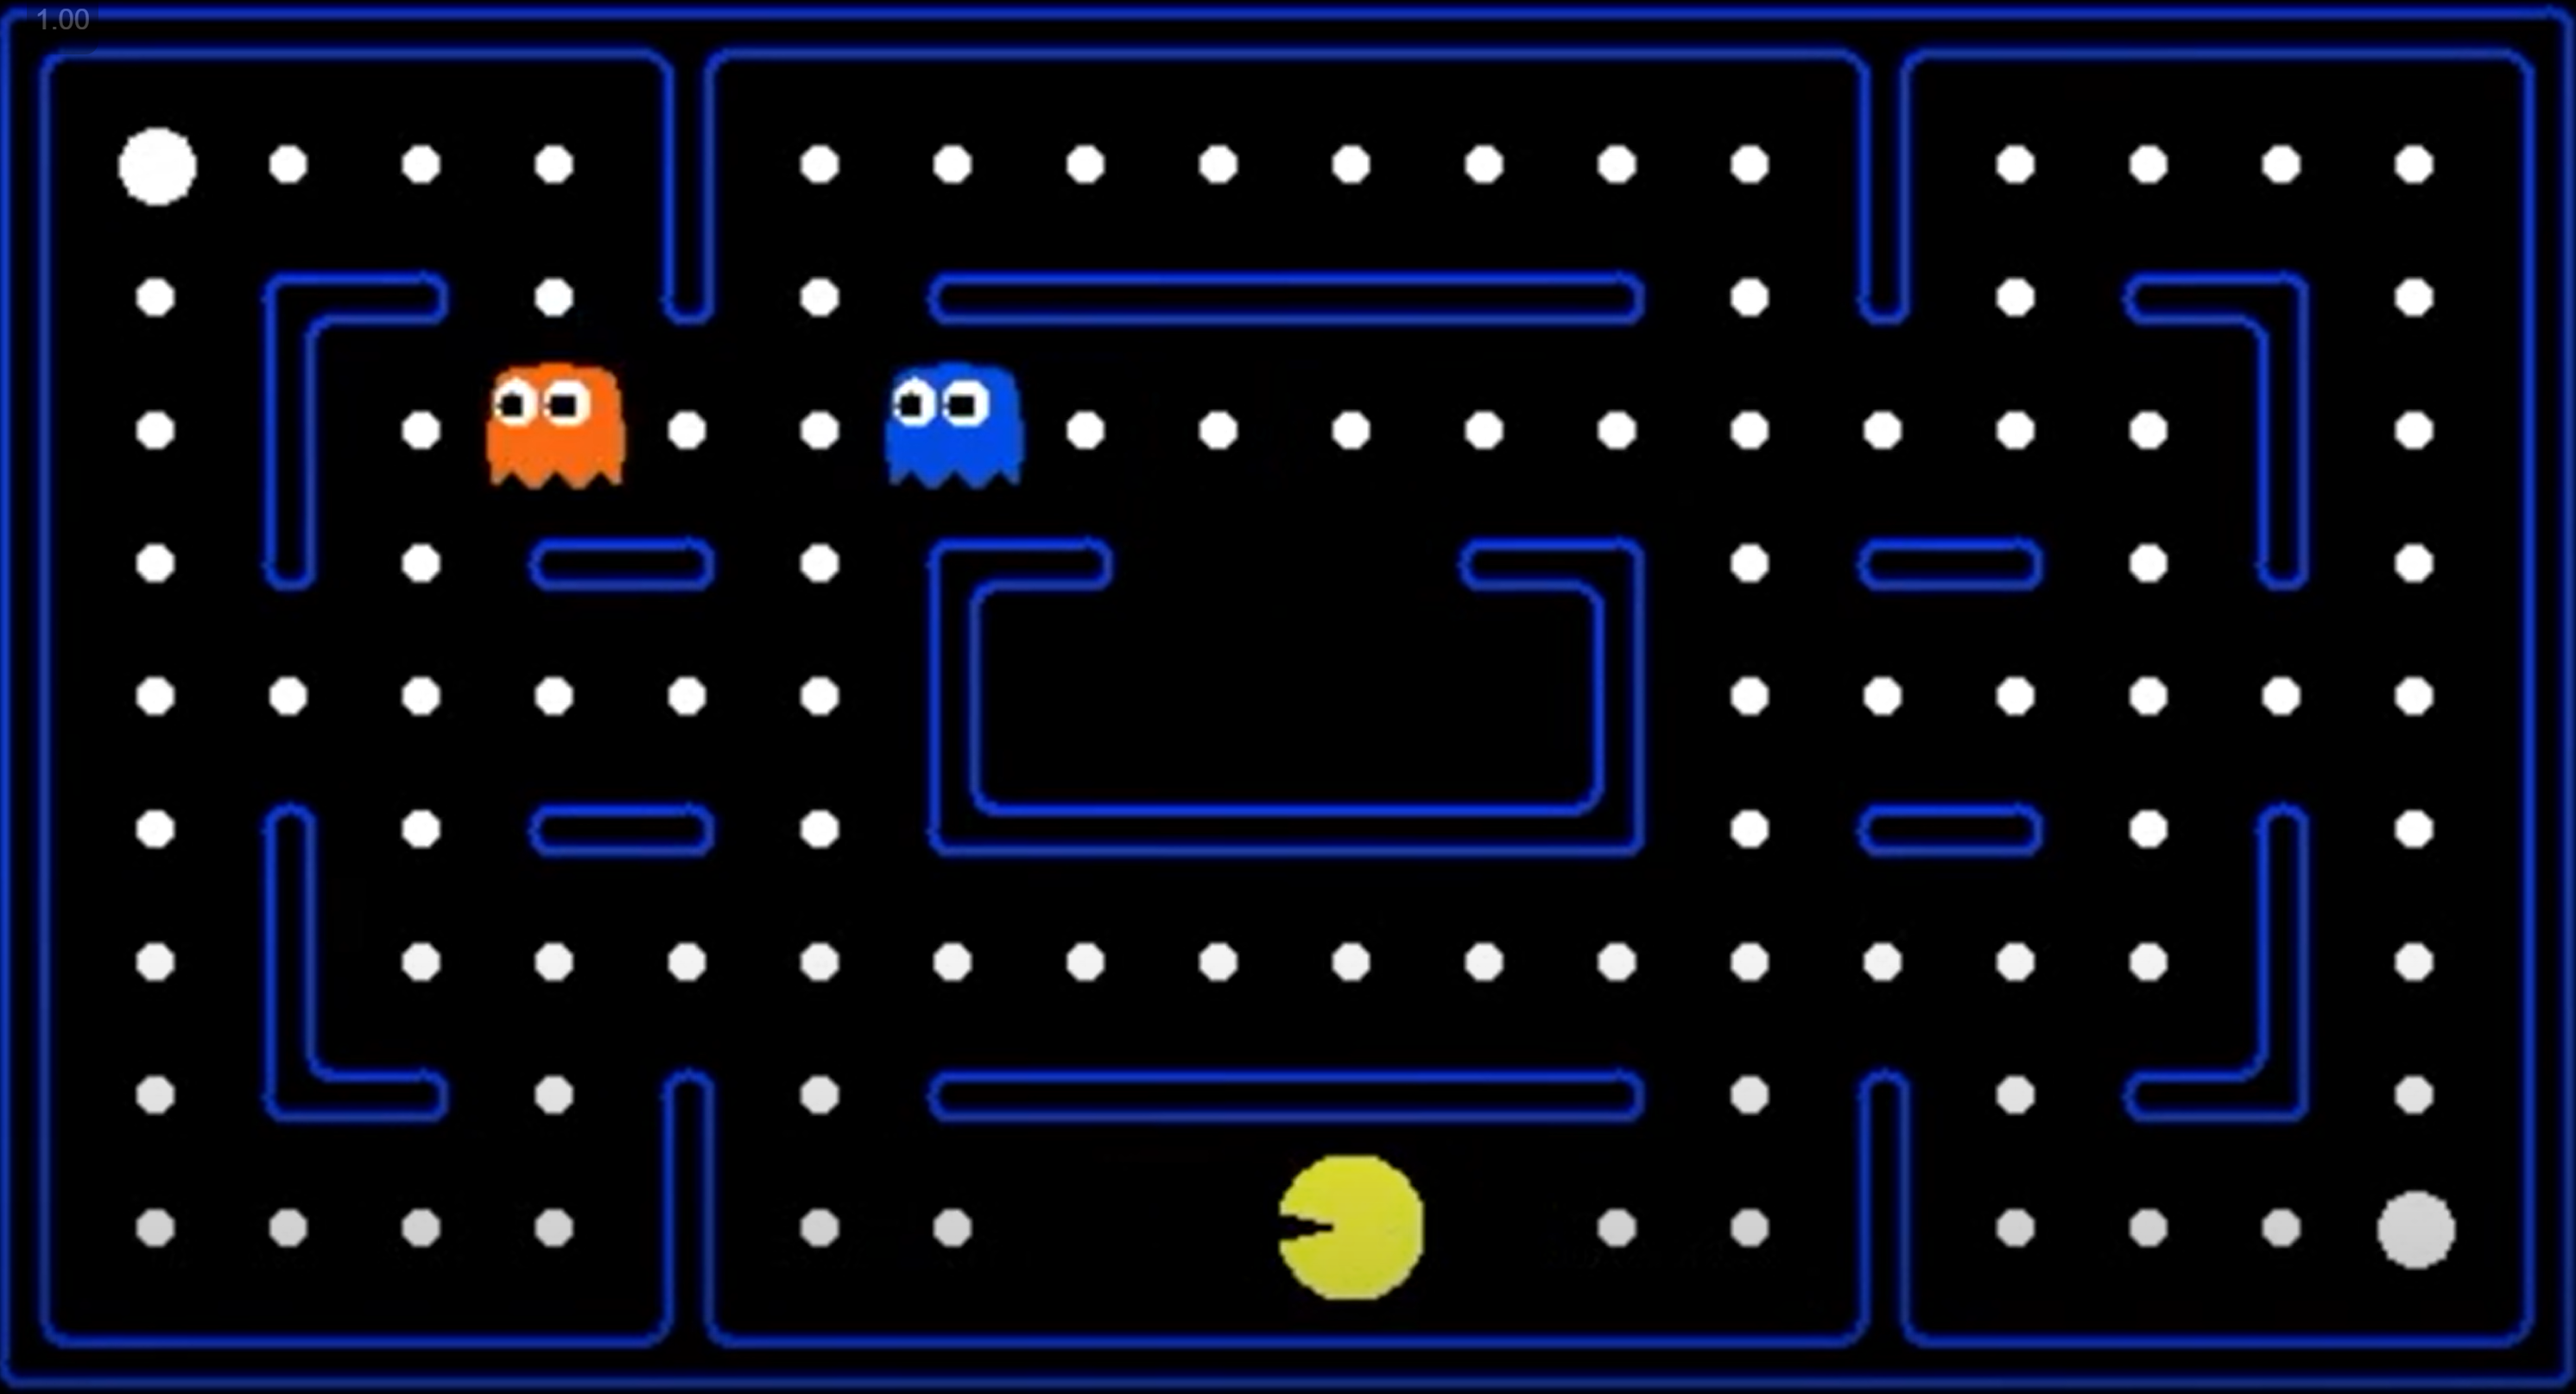
\includegraphics[keepaspectratio,
                     width=.8\paperwidth]{pacman.png}

                     \href{https://www.youtube.com/watch?v=QilHGSYbjDQ}{Deep Reinforcement Learning in Pac-man}
  \end{center}
\end{frame}

\note{Ok, so what we have in real world? Usually we do some action and get the result, and so we are learning gradually.}

\begin{frame}
  \frametitle{One more motivation}
  \framesubtitle{For example, we need to select the main page of a pizzeria website to attract the clients}

  \begin{columns}
      \begin{column}{.5\paperwidth}
        \begin{center}
          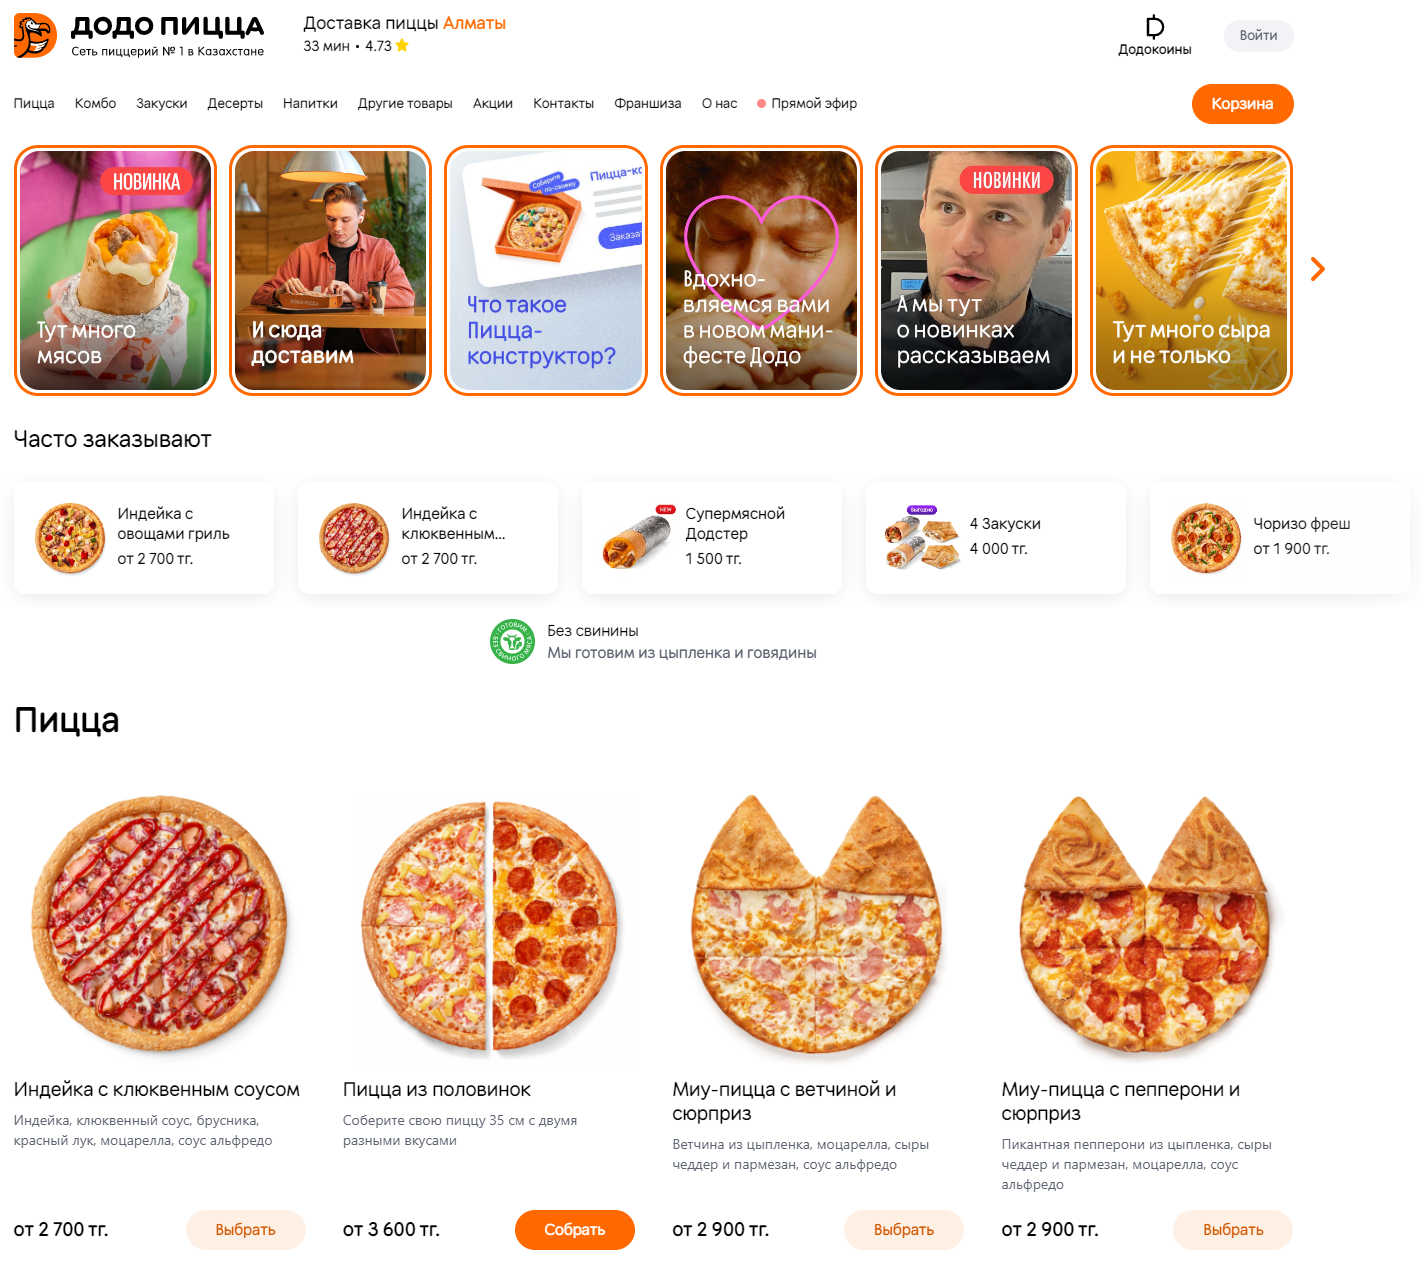
\includegraphics[keepaspectratio,
                           height=.45\paperheight]{pizza-1.png}
        \end{center}
      \end{column}
      \begin{column}{.5\paperwidth}
        \begin{center}
          
\includegraphics[keepaspectratio,
                           height=.4\paperwidth]{pizza-2.png}
        \end{center}
      \end{column}
  \end{columns}
\end{frame}

\note{And another one important example. Suppose you need to choose the most attractive design for the main page of a pizzeria website, but you don’t want to lose a lot of customers, time, money on experiments.}

\begin{frame}
  \frametitle{What approaches are there?}

  \begin{itemize}
    \pause
    \item A/B testing — many users see potentially bad options
    \pause
    \item multi-armed bandits — a special case of reinforcement learning
  \end{itemize}
\end{frame}

\note{In A/B testing you divide your customers on two groups (A and B), show them different versions of main page and then measure the results, the conversions and make your conclusions. And what is multi-armed bandits?}

\begin{frame}
  \frametitle{Bernoulli's one-armed bandit}

  \begin{center}
    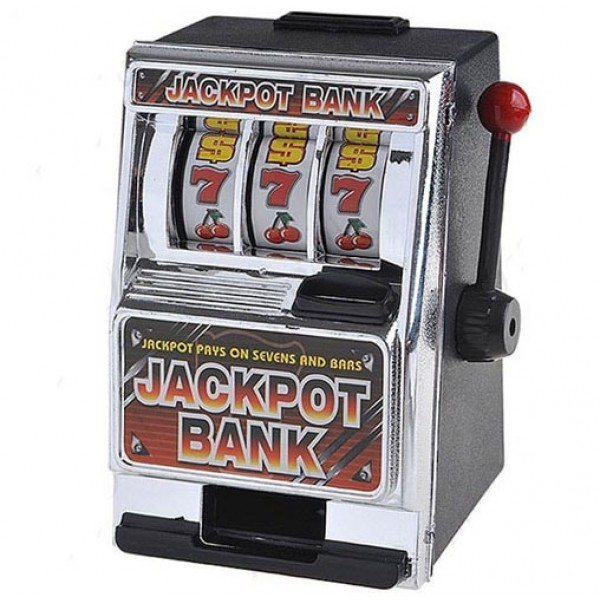
\includegraphics[keepaspectratio,
                     width=.5\paperwidth]{data-kopilkabandit.jpg}

    Probability of winning $\theta = 0.05$
  \end{center}
\end{frame}

\note{Let's begin from the one-armed bandit. So you pull the handle of a slot machine and you can win with some probability theta.}

\begin{frame}
  \frametitle{Multi-Armed Bandits}

  \begin{columns}
      \begin{column}{.25\paperwidth}
        \begin{center}
          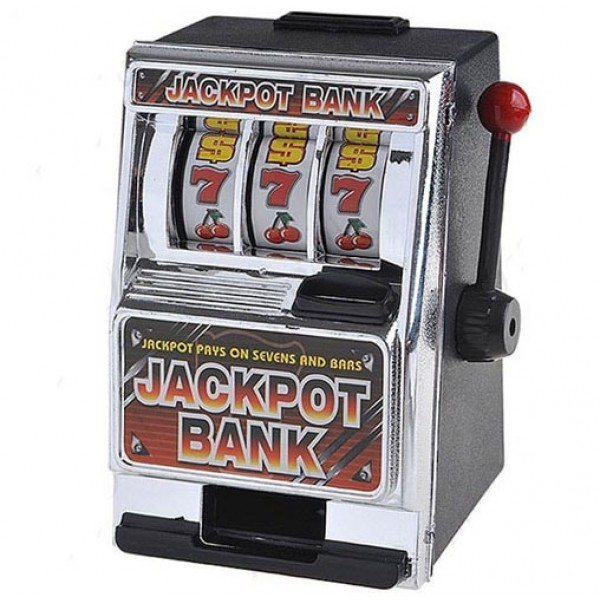
\includegraphics[keepaspectratio,
                           width=.2\paperwidth]{data-kopilkabandit.jpg}

        $\theta_1 = 0.02$
        \end{center}
      \end{column}
      \begin{column}{.25\paperwidth}
        \begin{center}
          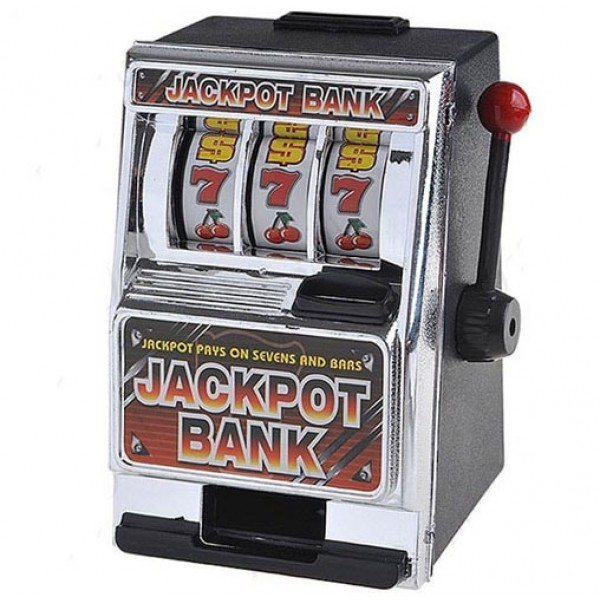
\includegraphics[keepaspectratio,
                           width=.2\paperwidth]{data-kopilkabandit.jpg}

          $\theta_2 = 0.01 (\min)$
        \end{center}
      \end{column}
      \begin{column}{.25\paperwidth}
        \begin{center}
          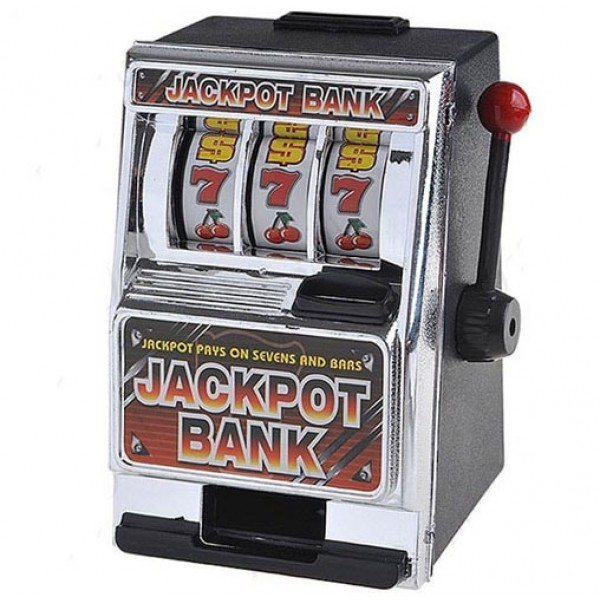
\includegraphics[keepaspectratio,
                           width=.2\paperwidth]{data-kopilkabandit.jpg}

        $\theta_3 = 0.05$
        \end{center}
      \end{column}
      \begin{column}{.25\paperwidth}
        \begin{center}
          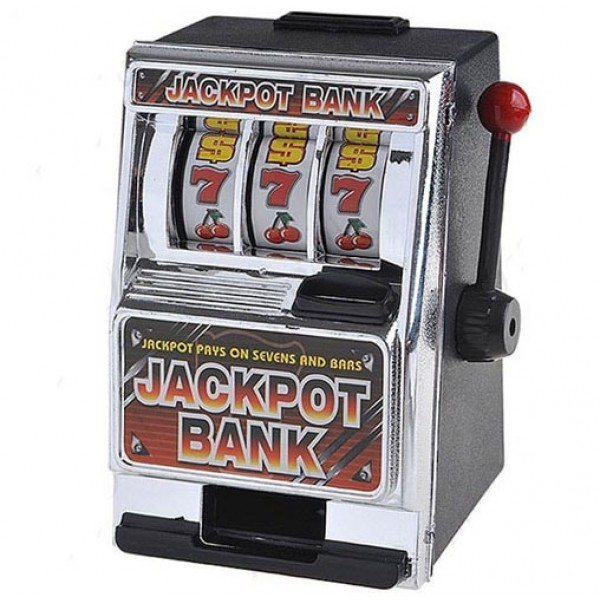
\includegraphics[keepaspectratio,
                           width=.2\paperwidth]{data-kopilkabandit.jpg}

           $\theta_4 = 0.1 (\max)$
        \end{center}
      \end{column}
  \end{columns}

  \vspace{1cm}
  We do not know the true probabilities, but we want to come up with a strategy that maximizes the payoff (reward)
\end{frame}

\note{In multi-armed bandits model you have several handles with some winning probabilities theta one, two and so on.}

\begin{frame}
  \frametitle{Mathematical statement of the problem}

  Given possible actions $$x_1, \dots, x_n$$

  \pause
  At the next iteration $t$, for each action $x^t_i$ performed, we get the answer $$ y^t_i \sim q(y|x^t_i, \Theta),$$

  \pause
  which brings us a {\bf reward} $$r_i^t = r(y^t_i)$$

  \pause
  There is an optimal action $x_{i^*}$ (sometimes $x_{i^*_t}$) $$\forall i:\ E(r_{i^*_t}^t) \geq E(r^t_i) $$

  \pause
  \begin{block}{Question}
    How to evaluate different strategies?
  \end{block}
\end{frame}

\note{Ok, now let's move on, to mathematical statement of the problem. ...}

\begin{frame}
  \frametitle{Measure of quality}

  \pause
  The quality measure of the multi-armed bandit algorithm $a$ is usually {\bf regret} $$ R(a) = \sum\limits_{t=1}^T \left(E(r_{i^*_t}^t) - E (r_{i^a_t}^t)\right)$$

  \vspace{1cm}
  Under synthetic conditions (when we know the probabilities), we can consider $$ E\left( R \right) = \int\limits_{\Theta} R(a)d\Theta$$
\end{frame}


\begin{frame}
   \frametitle{Multi-Armed Bandits possible applications}

   \begin{columns}
     \begin{column}{.4\paperwidth}
     Areas:
       \begin{itemize}
         \item advertising banners
         \item recommendations (goods, music, movies etc.)
         \item slot machines in the casino
       \end{itemize}
     \end{column}
     \begin{column}{.4\paperwidth}
       Approaches:
       \begin{itemize}
         \item Thompson sampling
         \item Upper Confidence Bound (UCB)
         \item $\varepsilon$-greedy strategy
       \end{itemize}
     \end{column}
   \end{columns}

   \vspace{1cm}
   \begin{block}{Note}
     The main difference from more general reinforcement learning approach is that there is no environment state in multi-armed bandits
   \end{block}
\end{frame}

\note{Ok, and what is the possible applications of multi-armed bandits? And there are models of implementing and optimizing the multi-armed bandits, but we won't discuss them in detail here.}

\begin{frame}
  \frametitle{Multi-Armed Bandits}
    \framesubtitle{Disadvantage}

   Do not take into account delayed effects

   For example, the effect of clickbait in advertising

   \pause
   \begin{center}
     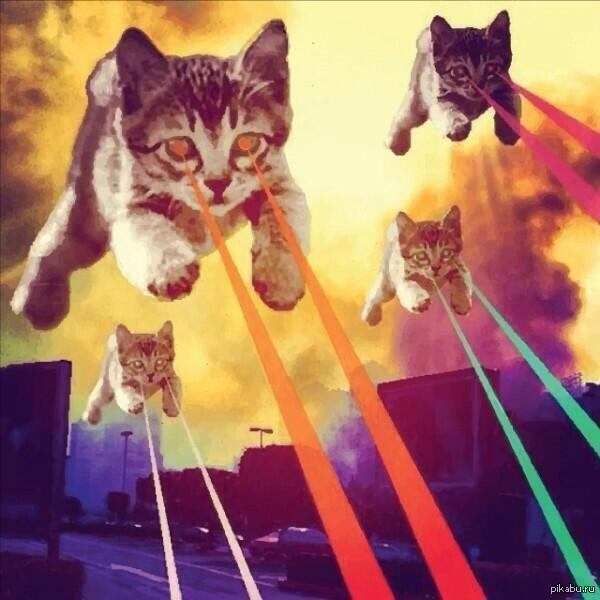
\includegraphics[keepaspectratio,
                      width=.45\paperwidth]{cats_invaders.jpg}

     SHOCK! Cats want to enslave us
   \end{center}
\end{frame}

\note{So you may increase your metrics for some short period of time by clickbait, but in the long run of course you will lose clients and money consequently.}

\begin{frame}
  \frametitle{Reinforcement Learning}
    \framesubtitle{Examples}

  \begin{center}
    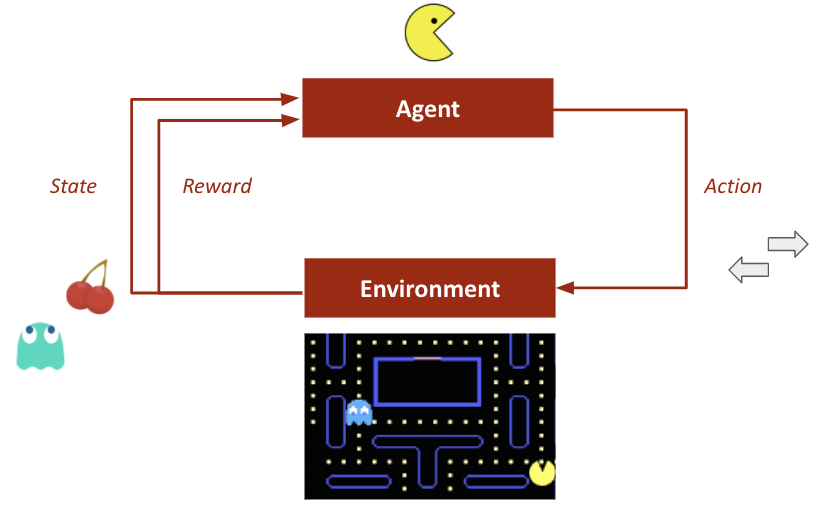
\includegraphics[keepaspectratio,
                     width=.7\paperwidth]{rl_scheme.png}
  \end{center}

  \begin{itemize}
    \pause
    \item robot control
    \pause
    \item (video) games
    \pause
    \item security management
  \end{itemize}
\end{frame}

\note{Let's go on to the Reinforcement Learning model.}

\begin{frame}
  \frametitle{Agent Model in a Changing Environment}

   \begin{columns}
     \begin{column}{.6\paperwidth}
       {\bf Definitions:}
       \begin{itemize}
         \item state $s \in S$
         \item agent action $a \in A$
         \item reward $r \in R$
         \item state transition dynamics

          $ P(s_{t+1} | s_t, a_t, \dots, s_{t-i}, a_{t-i}, \dots, s_0, a_0) $
         \item win function

          $$ r_{t} = r(s_t, a_t, \dots, s_0, a_0)$$
         \item total reward $R = \sum\limits_t r_t$
         \item agent policy $\pi (a | s)$
       \end{itemize}
     \end{column}
     \begin{column}{.3\paperwidth}
       {\bf Task:}
       $$ \pi (a | s): \mathbb{E}_\pi [R] \to \max $$
     \end{column}
   \end{columns}
\end{frame}

\note{So, more formally you have states, actions and rewards. And your task is to find optimal policy to maximize the total reward.}

\begin{frame}
  \frametitle{Cross-entropy method. Algorithm}

    Trajectory — $\left[s_0, a_0, s_1, a_1, s_2, \dots , a_{T-1}, s_T \right]$

   \vspace{1cm}
   {\bf Initialize} strategy model $\pi(a | s)$

   \vspace{1cm}
   {\bf Repeat}:
   \begin{itemize}
     \item play $N$ sessions
     \item choose the best $K$ of them and take their trajectories
     \item adjust $\pi(a | s)$ so that $s$ is able to maximize the probabilities of actions from the best trajectories
   \end{itemize}
\end{frame}

\note{The first simple algorithm to find appropriate policy is called cross-entropy method. Here you have some initialization, maybe random, as usual, then you play N sessions, choose best of them by your reward and update your strategy.}

\begin{frame}
  \frametitle{Training Example}

  \begin{center}
    \animategraphics[loop,width=0.6\paperwidth,autoplay]{4}{CartPole-v1-}{0}{157}
  \end{center}
\end{frame}


\begin{frame}
  \frametitle{Cross-entropy method. Implementation with a table}

    As a strategy model, we simply take a matrix $\pi$ of dimension $|S| \times |A|$

   $\pi(a | s) = \pi_{s,a}$

   after selecting the best trajectories, we obtain a set of pairs

   $$\text{Elite} = [(s_0, a_0), (s_1, a_1), (s_2, a_2), \dots, (s_H, a_H )]$$

   and maximize the likelihood

   $$ \pi_{s,a} = \frac{\sum\limits_{s_t, a_t \in \text{Elite}} [s_t = s][a_t = a]}{\sum\limits_{s_t, a_t \ in \text{Elite}} [s_t = s]}$$
\end{frame}


\begin{frame}
  \frametitle{There is a problem..}

  \pause
  that there are a lot of states:
  \begin{center}
    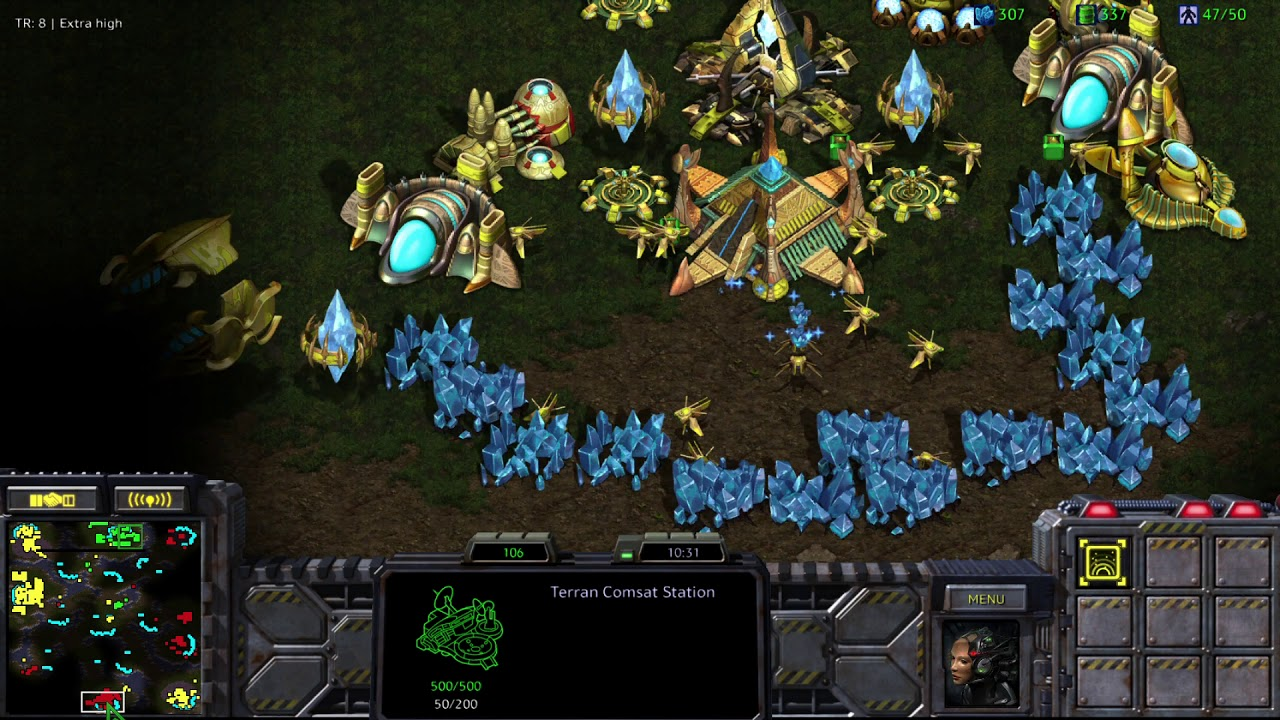
\includegraphics[keepaspectratio,
                     width=.85\paperwidth]{starcraft3.jpg}
  \end{center}
\end{frame}

\note{So the problem is, that we can not even store in memory the whole table of states.}

\begin{frame}
\frametitle{Approximate cross-entropy methods}

    Possible solutions:
    \begin{itemize}
      \item split the state space into sections and treat them as states
      \pause
      \item get probabilities from $\pi_\theta (a | s)$ machine learning model: linear model, neural network, random forest
      \pause
      \item often these probabilities need to be further specified later
    \end{itemize}
\end{frame}

\note{So people invented Approximate cross-entropy methods.}

\begin{frame}
  \frametitle{Approximate cross-entropy method}
    \framesubtitle{Example}

   \begin{itemize}
     \pause
     \item As a strategy model, we take just a neural network $\pi_\theta$

     \pause
     \item Initialize with random weights

     \pause
     \item At each iteration, after selecting the best trajectories, we obtain a set of pairs
       $$\text{Elite} = [(s_0, a_0), (s_1, a_1), (s_2, a_2), \dots, (s_H, a_H )]$$

     \pause
     \item and perform optimization
       $$ \pi = \arg\max\limits_\theta \sum\limits_{s_i, a_i \in \text{Elite}} \log \pi(a_i|s_i) = \arg\max\limits_\theta \mathscr{ L}(\theta)$$

     \pause
     \item that is
       $$ \theta_{t+1} = \theta_{t} + \alpha \nabla \mathscr{L}(\theta) $$
   \end{itemize}
\end{frame}


\begin{frame}
  \frametitle{Why is it called cross-entropy method?}

   \begin{align*}
     KL(p_1(x) \| p_2(x)) = E_{x \sim p_1(x)} \log \frac{p_1(x)}{p_2(x)} = \\
     =
     \underbrace{E_{x \sim p_1(x)} \log {p_1(x)}}_{
       \text{entropy}
     }-
     \underbrace{E_{x \sim p_1(x)} \log {p_2(x)}}_{
     \text{cross entropy}
     }
   \end{align*}
\end{frame}


\begin{frame}
  \frametitle{Disadvantages of the cross-entropy method}

    \begin{itemize}
      \pause
      \item it is unstable for small samples
      \pause
      \item in the case of a non-deterministic environment, it chooses lucky cases (random played in favor of the agent)
      \pause
      \item it is focusing on behavior in simple states
      \pause
      \item it ignores a lot of information
      \pause
      \item there are tasks in which the end never comes (stock market game)
   \end{itemize}
\end{frame}

\note{... So we need to correct these shortcomings.}

\begin{frame}
  \frametitle{Q-Learning}

  \begin{itemize}
    \item sometimes it is not necessary to finish the game to evaluate the effectiveness of the strategy
    \item the effect of the action may appear later
   \end{itemize}
\end{frame}


\begin{frame}
  \frametitle{Markov Decision Process}

\begin{columns}
    \begin{column}{.6\paperwidth}
      {\bf Definitions:}
      \begin{itemize}
        \item state $s \in S$
        \item agent action $a \in A$
        \item reward $r \in R$
        \item transition dynamics

         $ P(s_{t+1} | s_t, a_t, \dots, s_{t-i}, a_{t-i}, \dots, s_0, a_0) = P(s_{t+1} | s_t, a_t)$
         {\bf (Markov's assumption)}

        \item win function

         $$ r_{t} = r(s_t, a_t)$$ {\bf (Markov's assumption)}
        \item total reward $R = \sum\limits_t r_t $
      \end{itemize}
    \end{column}
    \begin{column}{.3\paperwidth}

      \begin{itemize}
        \item agent policy

        $$ \pi (a | s) $$
      \end{itemize}
      {\bf Task:}
      $$ \pi (a | s): \mathbb{E}_\pi [R] \to \max $$
    \end{column}
  \end{columns}
\end{frame}

\note{Here we have Markov's assumption, which is actually not so strong, as we could expect. For example it is true in chess and Starcraft also. Only your current state determines everything, and not the history of the game.}

\begin{frame}
  \frametitle{Important definitions}
    Average absolute win:
    $$ \mathbb{E}_{s_0 \sim p(s_0),} \mathbb{E}_{a_0 \sim \pi(a|s_0),} \mathbb{E}_{s_1, r_0 \sim P (s^\prime,r|s, a)} \dots \left[r_0 + r_1 + \dots + r_T \right]$$

    State value function:
    $$ V^{\pi} (s) = \mathbb{E}_\pi [R_t|s_t = s] =
    \mathbb{E}_\pi \left[\sum\limits_{k=0}^\infty \gamma^k r_{t+k+1} | s_t = s\right]$$

    Action value function in state:
    $$ Q^{\pi} (s, a) = \mathbb{E}_\pi [R_t|s_t = s, a_t = a] =
    \mathbb{E}_\pi \left[\sum\limits_{k=0}^\infty \gamma^k r_{t+k+1} | s_t = s, a_t = a \right]$$

    where $\pi$ is the strategy followed by the agent, $\gamma \in [0, 1]$
\end{frame}


\begin{frame}
  \frametitle{TD-training}
    \framesubtitle{temporal difference}

    We arbitrarily initialize the function $V(s)$ and the strategy $\pi$

    Then we repeat
    \begin{itemize}
      \item initialize $s$
      \item for each agent step
        \begin{itemize}
          \item select $a$ by strategy $\pi$
          \item do action $a$, get result $r$ and next state $s^\prime$
          \item update function $V(s)$ by formula
          $$ V(s) = V(s) + \alpha \left(r + \gamma V(s^\prime) - V(s) \right)$$
          \item go to the next step by assigning $s := s^\prime$
        \end{itemize}
    \end{itemize}
\end{frame}

\note{The amazing fact is, that temporal difference training works.}


\begin{frame}
  \frametitle{Bellman Equation}
    \framesubtitle{for the optimal value function $Q^*$}

    $$ Q^* (s,a) = \mathbb{E}_\pi \left[r_t + \gamma \max\limits_{a^\prime} Q^* (s_{t+1},a^\prime) \mid s_t = s, a_t = a \right]$$

    \vspace{1cm}
    \begin{block}{Note}
      The greedy strategy $\pi$ with respect to $Q^*(s,a)$ ``choose the action that maximizes the Bellman equations'' is optimal.
    \end{block}
\end{frame}


\begin{frame}
  \frametitle{State utility recalculation}

    $$V(s) = \max\limits_a [r(s, a) + \gamma V(s^\prime (s, a))]$$

    \vspace{0.5cm}
    that is, with probabilistic transitions
    $$V(s) = \max\limits_a [r(s, a) + \gamma \mathbb{E}_{s^\prime \sim P(s^\prime | s, a)} V(s^ \prime)]$$

    \vspace{0.5cm}
    Iterative State Utility Recalculation Formula
    \begin{align*}
      \forall s \ V_0(s) &= 0 \\
      V_{i+1}(s) &= \max\limits_a [r(s, a) + \gamma \mathbb{E}_{s^\prime \sim P(s^\prime | s, a)} V_{i}(s^\prime)]
    \end{align*}
    \pause
    \begin{block}{Note}
      To use this formula in practice,
      we need to know the transition probabilities $P(s^\prime| s, a)$
    \end{block}
\end{frame}


\begin{frame}
  \frametitle{Utility of an action}

    $$Q(s, a) = r(s, a) + \gamma V(s^\prime)$$

    The strategy of the game is defined as follows

    $$\pi(s) : \arg\max\limits_a Q(s, a)$$

    \pause
    Again due to stochasticity

    $$Q(s, a) = \mathbb{E}_{s^\prime} [r(s, a) + \gamma V(s^\prime)]$$

    It is possible to estimate the expected value without an explicit distribution, using the Monte Carlo method and averaging over the outcomes:

    $$Q(s_t, a_t) \leftarrow \alpha \left(r_t+\gamma \max\limits_a Q(s_{t+1}, a) \right)
    + (1-\alpha) Q(s_{t}, a_{t})$$
\end{frame}


\begin{frame}
  \frametitle{DQN (Deep Q-Learning Network)}

  Environment is Atari game emulator, each frame $210\times 160pix, \ 128col$
  \begin{center}
     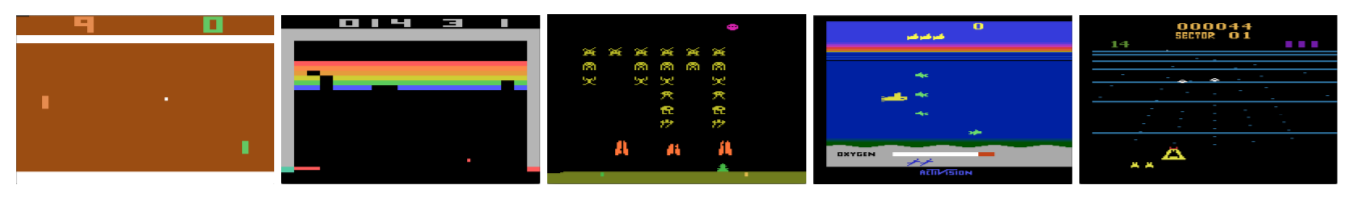
\includegraphics[keepaspectratio,
                      width=.95\paperwidth]{atari_games.png}
  \begin{columns}
      \begin{column}{.15\paperwidth}
      Pong
      \end{column}
      \begin{column}{.15\paperwidth}
      Breakout
      \end{column}
      \begin{column}{.15\paperwidth}
      Space Invaders
      \end{column}
      \begin{column}{.15\paperwidth}
      Seaquest
      \end{column}
      \begin{column}{.15\paperwidth}
      Beam Rider
      \end{column}
  \end{columns}
\end{center}
   
   \pause
   \textbf{s} states: 4 consecutive frames compressed to $84 \times 84$

   Actions \textbf{a}: from 4 to 18, depending on the game

   \textbf{r} rewards: current in-game SCORE

   Value function $Q(s, a; w)$: 

   ConvNN with input $s$ and $|A|$ outputs

  \vspace{0.5cm}
  \noindent\rule{8cm}{0.4pt}

  {\footnotesize
  {\it V.Mnih et al.} (DeepMind). Playing Atari with deep reinforcement learning. 2013}
\end{frame}

\note{Ok, and the last reinforcement learning model in our lecture is the Deep Q-Learning Network.}

\begin{frame}
  \frametitle{DQN Method}

  \pause
  Saves trajectories $(s_t, a_t, r_t)_{t=1}^T$ in replay memory for repeated experience replay

  \pause
  \vspace{0.2cm}
  Gets approximation of the optimal value function $Q(s_t, a_t)$ for fixed current network parameters ${\color{red} w_t}$

  $$y_t =
  \left\{ \begin{aligned}
  &r_t, \text{ if state } s_{t+1} \text{ terminal } \\
  &r_t + \gamma \max_a Q(s_{t+1}, a; {\color{red} w_t}), \text{ otherwise}
  \end{aligned}\right.
  $$

  \pause
  Evaluates loss function for training the neural network model $Q(s, a; w)$:

  $$ \mathscr{L} (w) = (Q(s_t, a_t; w) - y_t)^2 $$

  with stochastic gradient SGD (by mini-batches of length 32):

  $$ w_{t+1} = w_{t} - \eta \left(Q(s_t, a_t; w_t) - y_t\right) \nabla_w Q(s_t, a_t; w_t) $$
\end{frame}


\begin{frame}
  \frametitle{Network architecture for the value function}
  \begin{center}
    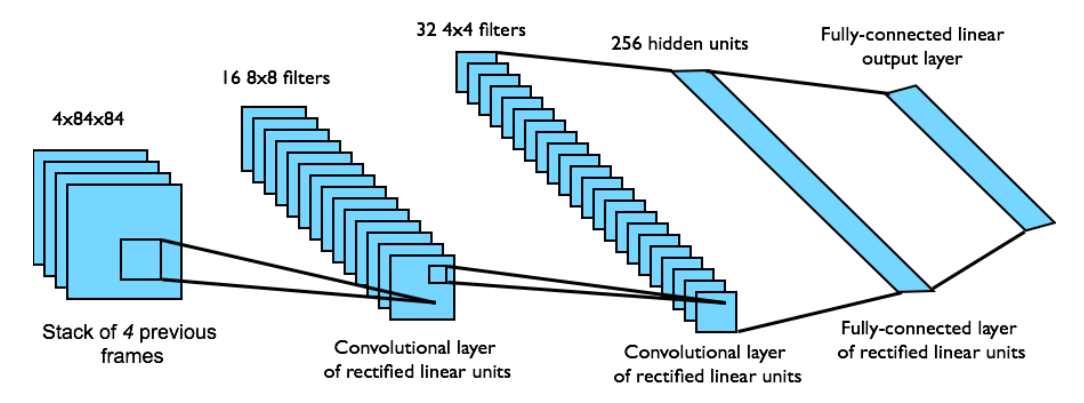
\includegraphics[keepaspectratio,
                     width=.85\paperwidth]{dql-cnn-arch.png}
  \end{center}
\end{frame}

\note{Here your see actual CNN structure for Atari game — quite simple, isn't it? And I think you know what happened next :)}

{ % all template changes are local to this group.
    \setbeamertemplate{navigation symbols}{}
    \begin{frame}<article:0>[plain]
        \begin{tikzpicture}[remember picture,overlay]
            \node[at=(current page.center)] {
                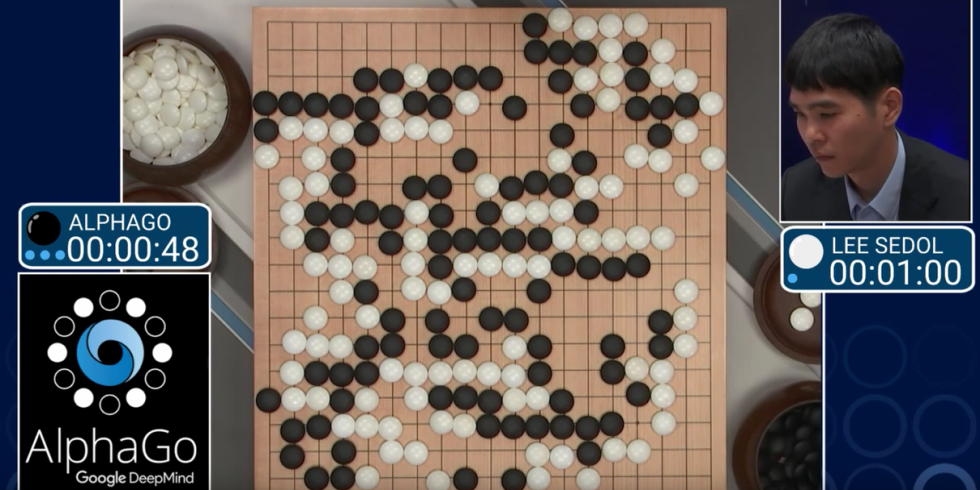
\includegraphics[keepaspectratio,
                                 width=\paperwidth,
                                 height=\paperheight]{alpha_go.png}
            };
        \end{tikzpicture}
     \end{frame}
}


{ % all template changes are local to this group.
    \setbeamertemplate{navigation symbols}{}
    \begin{frame}<article:0>[plain]
        \begin{tikzpicture}[remember picture,overlay]
            \node[at=(current page.center)] {
                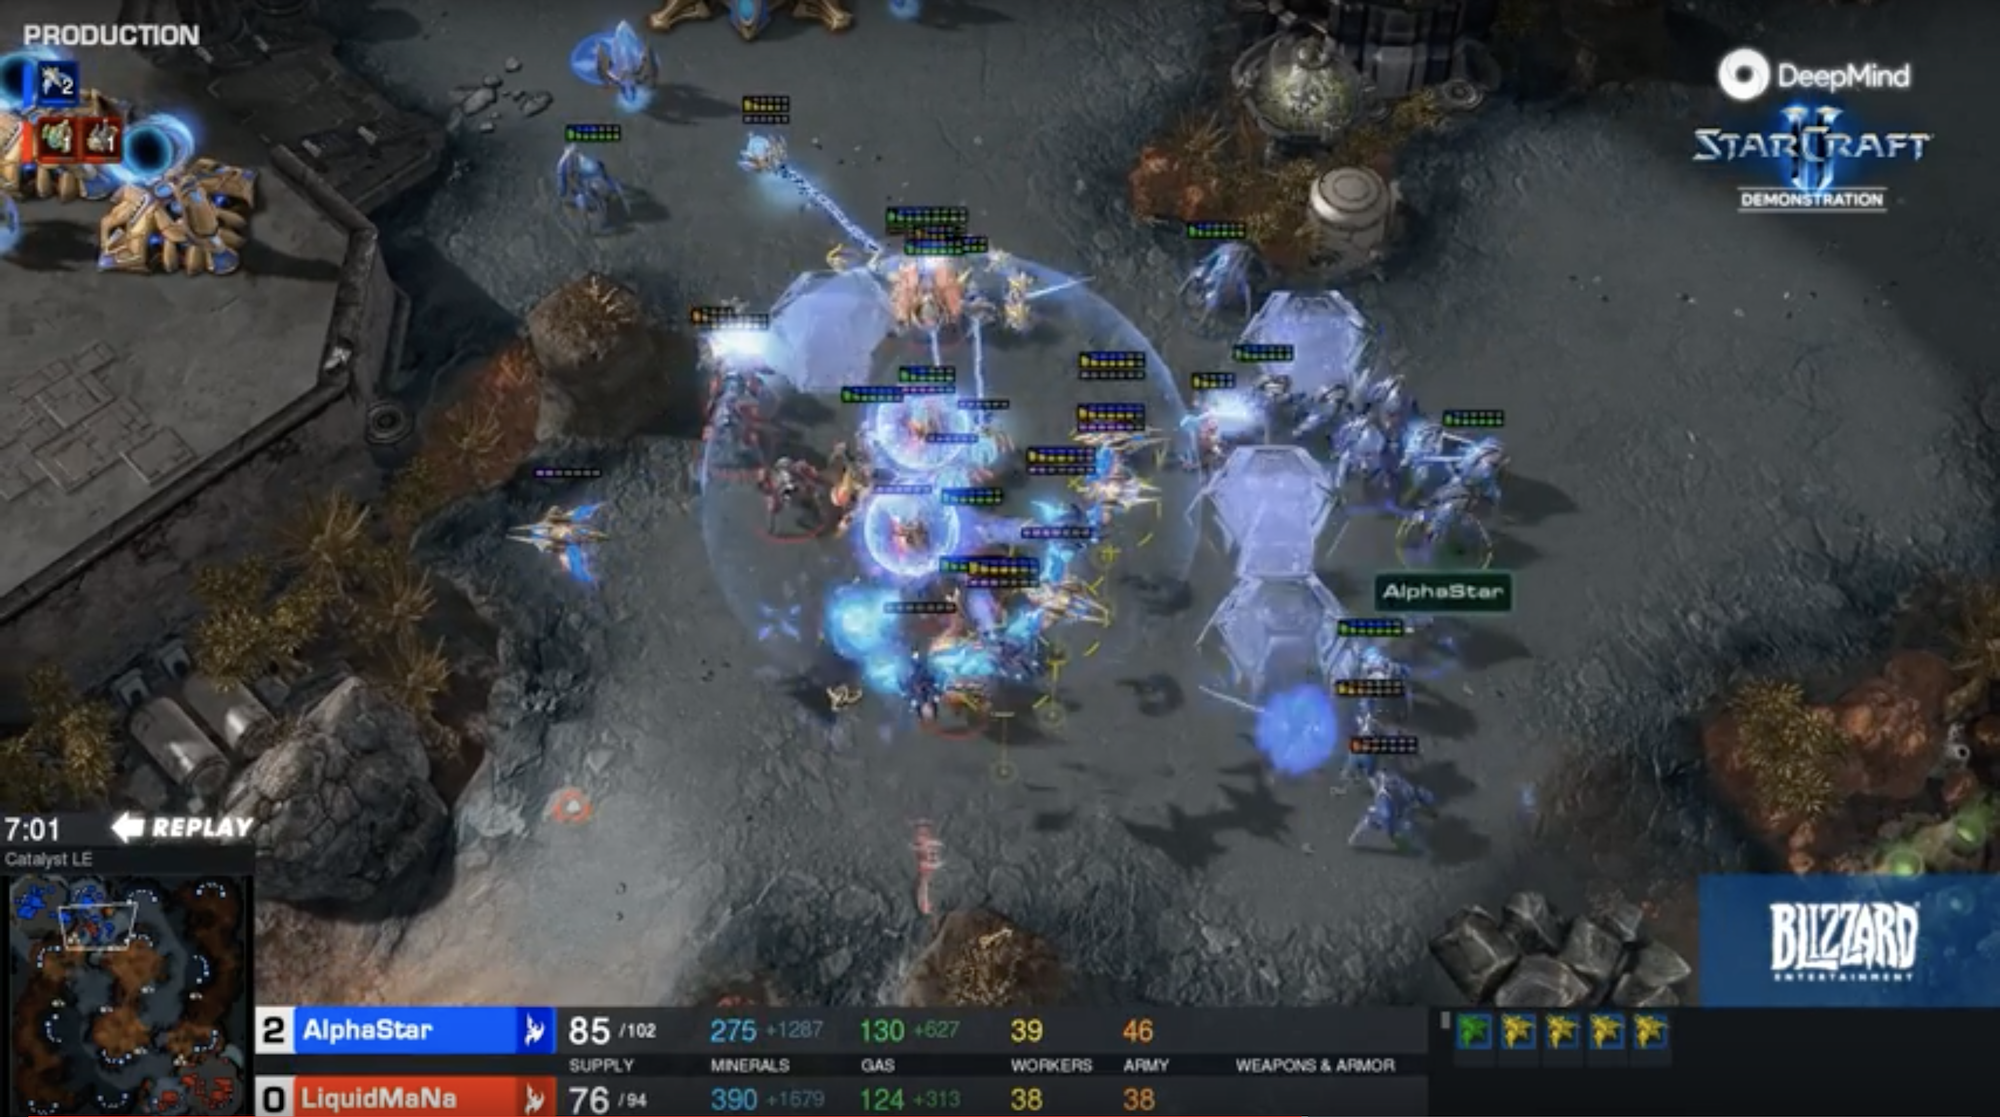
\includegraphics[keepaspectratio,
                                 width=\paperwidth,
                                 height=\paperheight]{AI-AlphaStar-StarCraft-II.png}
            };
        \end{tikzpicture}
     \end{frame}
}


\begin{frame}[t]
\frametitle{Summary}

  \begin{itemize}
    \item we got acquainted with the reinforcement learning problem statement
    \item touched a little multi-armed bandits
    \item got acquainted with the methods of cross-entropy, TD-learning and Q-learning
    \item discussed Deep Q-learning Network
    \item did NOT discuss the central method in robotics — policy gradient descent
  \end{itemize}

  \pause
  What else can you see?

  \begin{itemize}
    \item main book on the topic: \href{https://web.stanford.edu/class/psych209/Readings/SuttonBartoIPRLBook2ndEd.pdf}{Reinforcement Learning: An Introduction}, Richard S. Sutton and Andrew G. Barto
    \item \href{https://spinningup.openai.com/en/latest}{Educational resource on RL produced by OpenAI}
    \item Yuxi Li. Resources for Deep Reinforcement Learning. 2018
    \item \href{https://www.deepmind.com/learning-resources/introduction-to-reinforcement-learning-with-david-silver}{Intro to RL with David Silver}
  \end{itemize}
\end{frame}

\end{document}
